\documentclass[11pt]{aghdpl}
% \documentclass[en,11pt]{aghdpl}  % praca w języku angielskim

% Lista wszystkich języków stanowiących języki pozycji bibliograficznych użytych w pracy.
% (Zgodnie z zasadami tworzenia bibliografii każda pozycja powinna zostać utworzona zgodnie z zasadami języka, w którym dana publikacja została napisana.)
\usepackage[english,polish]{babel}

% Użyj polskiego łamania wyrazów (zamiast domyślnego angielskiego).
\usepackage{polski}

\usepackage[utf8]{inputenc}

% dodatkowe pakiety

\usepackage{mathtools}
\usepackage{float}
\usepackage{amsfonts}
\usepackage{amsmath}
\usepackage{textcomp}
\usepackage{amsthm}

% --- < bibliografia > ---

\usepackage[
style=numeric,
sorting=none,
%
% Zastosuj styl wpisu bibliograficznego właściwy językowi publikacji.
language=autobib,
autolang=other,
% Zapisuj datę dostępu do strony WWW w formacie RRRR-MM-DD.
urldate=iso8601,
% Nie dodawaj numerów stron, na których występuje cytowanie.
backref=false,
% Podawaj ISBN.
isbn=true,
% Nie podawaj URL-i, o ile nie jest to konieczne.
url=false,
%
% Ustawienia związane z polskimi normami dla bibliografii.
maxbibnames=3,
% Jeżeli używamy BibTeXa:
backend=bibtex
]{biblatex}

\usepackage{csquotes}
% Ponieważ `csquotes` nie posiada polskiego stylu, można skorzystać z mocno zbliżonego stylu chorwackiego.
\DeclareQuoteAlias{croatian}{polish}

\addbibresource{bibliografia.bib}

% Nie wyświetlaj wybranych pól.
%\AtEveryBibitem{\clearfield{note}}


% ------------------------
% --- < listingi > ---

% Użyj czcionki kroju Courier.
\usepackage{courier}

\usepackage{listings}
\lstloadlanguages{TeX}

\lstset{
	literate={ą}{{\k{a}}}1
           {ć}{{\'c}}1
           {ę}{{\k{e}}}1
           {ó}{{\'o}}1
           {ń}{{\'n}}1
           {ł}{{\l{}}}1
           {ś}{{\'s}}1
           {ź}{{\'z}}1
           {ż}{{\.z}}1
           {Ą}{{\k{A}}}1
           {Ć}{{\'C}}1
           {Ę}{{\k{E}}}1
           {Ó}{{\'O}}1
           {Ń}{{\'N}}1
           {Ł}{{\L{}}}1
           {Ś}{{\'S}}1
           {Ź}{{\'Z}}1
           {Ż}{{\.Z}}1,
	basicstyle=\footnotesize\ttfamily,
}

% ------------------------

\AtBeginDocument{
	\renewcommand{\tablename}{Tabela}
	\renewcommand{\figurename}{Rys.}
}

% ------------------------
% --- < tabele > ---

\usepackage{array}
\usepackage{tabularx}
\usepackage{multirow}
\usepackage{booktabs}
\usepackage{makecell}
\usepackage[flushleft]{threeparttable}

% defines the X column to use m (\parbox[c]) instead of p (`parbox[t]`)
\newcolumntype{C}[1]{>{\hsize=#1\hsize\centering\arraybackslash}X}


%---------------------------------------------------------------------------

\author{Szymon Nowak}
\shortauthor{Sz. Nowak}

%\titlePL{Przygotowanie bardzo długiej i pasjonującej pracy dyplomowej w~systemie~\LaTeX}
%\titleEN{Preparation of a very long and fascinating bachelor or master thesis in \LaTeX}

\titlePL{Sterowanie funkcjami inteligentnego budynku w oparciu o mapy przepływu użytkowników}
\titleEN{}


\shorttitlePL{Sterowanie funkcjami inteligentnego budynku} % skrócona wersja tytułu jeśli jest bardzo długi
\shorttitleEN{}

\thesistype{Praca dyplomowa inżynierska}
%\thesistype{Master of Science Thesis}

\supervisor{dr Dariusz Pałka}
%\supervisor{Marcin Szpyrka PhD, DSc}

\degreeprogramme{Informatyka}
%\degreeprogramme{Computer Science}

\date{2017}

\department{Katedra Informatyki Stosowanej}
%\department{Department of Applied Computer Science}

\faculty{Wydział Elektrotechniki, Automatyki,\protect\\[-1mm] Informatyki i Inżynierii Biomedycznej}
%\faculty{Faculty of Electrical Engineering, Automatics, Computer Science and Biomedical Engineering}

\acknowledgements{Składam serdeczne podziękowania dla promotora, dra Dariusza Pałki, za pomocne uwagi i cenne wskazówki, udzielane podczas pisania pracy, narzeczonej za cierpliwość i wyrozumiałość oraz rodzinie za wsparcie}


\setlength{\cftsecnumwidth}{10mm}

%---------------------------------------------------------------------------
\setcounter{secnumdepth}{4}
\brokenpenalty=10000\relax

\begin{document}

\titlepages

% Ponowne zdefiniowanie stylu `plain`, aby usunąć numer strony z pierwszej strony spisu treści i poszczególnych rozdziałów.
\fancypagestyle{plain}
{
	% Usuń nagłówek i stopkę
	\fancyhf{}
	% Usuń linie.
	\renewcommand{\headrulewidth}{0pt}
	\renewcommand{\footrulewidth}{0pt}
}

\setcounter{tocdepth}{2}
\tableofcontents
\clearpage

\chapter{Wprowadzenie}
\label{cha:wprowadzenie}

Brak wprowadzenia.

%---------------------------------------------------------------------------

\section{Cele pracy}
\label{sec:celePracy}

Brak celu.

%---------------------------------------------------------------------------

\section{Zawartość pracy}
\label{sec:zawartoscPracy}

Brak zawartości.



















\chapter{Określanie lokalizacji}
\label{cha:lokalizacja}
\section{Lokalizacja użytkownika}
Lokalizację użytkownika w systemie określa się na podstawie odległości od punktów, których współrzędne w przestrzeni trójwymiarowej są znane. Są to głównie routery i Beacony, jednak może się zdarzyć, że takim punktem staje się również inny użytkownik. Współrzędne użytkownika można obliczyć, dokonując pomiarów wskaźnika mocy \textit{RSSI}, podając siłę sygnałów odebranych przez otaczające go urządzenia i obliczając na ich podstawie dystans \cite{RSC}.
\section{Trilateracja}
Powszechnie wykorzystywanym sposobem obliczenia lokalizacji użytkownika na podstawie dystansu do znanych punktów, jest trilateracja \cite{MS}. Metoda ta polega na przedstawieniu dystansu dzielącego punkt od nadajników w postaci okręgi (lub sfery w przypadku, gdy określamy lokalizację w trzech wymiarach). Następnie, należy wyznaczyć współrzędne punktu przecięcia okręgów \cite{MS}. Wyznaczony punkt jest lokalizacją odbiornika, dla którego dokonywaliśmy obliczenia.
\begin{figure}[H]			
	\centering
	\caption{Wizualizacja modelu trilateracji}
	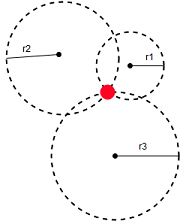
\includegraphics{trilateracja}
\end{figure}
Współrzędną punktu można obliczyć na podstawie wzoru:
\begin{equation}
\left\{
\begin{array}{l}
(x_p-x_1)^2 + (y_p - y_1)^2 = r_1^2\\
(x_p-x_2)^2 + (y_p - y_2)^2 = r_2^2\\
(x_p-x_3)^2 + (y_p - y_3)^2 = r_3^2
\end{array}
\right.
\end{equation}
gdzie:
\begin{itemize}
	\item $x_p$, $y_p$ to współrzędne obliczanego odbiornika
	\item $x_1$, $y_1$, $x_2$, $y_2$, $x_3$, $y_3$ to współrzędne znanych punktów
	\item $r_1$, $r_2$, $r_3$ to odległości między punktem obliczanym, a punktami o znanych współrzędnych
\end{itemize}
Ta metoda lokalizowania użytkownika w przestrzeni ma jedną, bardzo ważną wadę, która wyklucza jej wykorzystanie w tworzonym systemie - nie potrafi się dostosować do błędów pomiarowych, których w przypadku określania lokalizacji przy użyciu sygnałów radiowych, jest dużo. Aby wyznaczone lokalizacje użytkowników w sposób zbliżony odwzorowywały rzeczywiste położenie, algorytm obliczający musiał być bardziej odporny na błędy pomiarowe \cite{MT}.
\section{Lokalizacja jako funkcja probabilistyczna Gaussa}
Z racji tego, iż mierzony sygnał, odbierany przez odbiornik, ulega zniekształceniom i odbiciom, określenie dystansu między transmiterem, a odbiorcą w sposób liniowy jest niezgodne z fizycznymi zachowaniami sygnału. Siła sygnału oraz straty wywołane przez zniekształcenia i odbicia, określone są w jednostce dB. Wynika z tego, że najlepszym przybliżeniem zmian siły sygnału może być funkcja Gaussa \cite{GMBF}. Zamiast określać konkretne położenie użytkownika, w pracy zastosowane będzie podejście, które pozwoli na przedstawienie jego lokalizacji jako prawdopodobieństwo położenia.\\
\subsection{Funkcja probabilistyczna Gaussa}
Funkcja probabilistyczna Gaussa jest to krzywa w kształcie dzwonu, symetryczna względem średniej $\mu$ oraz uzyskująca wartość maksymalną w punkcie $\frac{1}{\sqrt{2\pi}\sigma}$.
Określa się ją za pomocą wzoru:
\begin{equation}
F(x) = \frac{1}{\sigma\sqrt{2\pi}}e^{\left(\frac{-(x-\mu)^2}{2\sigma^2}\right)}
\end{equation}
Zmienne $\mu$ będąca średnią, oraz $\sigma$ będąca odchyleniem standardowym, w pełni opisują tą funkcję \cite{MIR}.
\begin{figure}[H]			
	\centering
	\caption{Wykres funkcji Gaussa dla różnych wartości parametrów}
	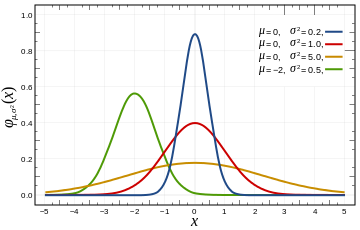
\includegraphics{funkcja_Gaussa}
\end{figure}
Funkcja Gaussa jest szeroko wykorzystywana w statystyce. W elektronice, korzysta się z niej podczas charakteryzowania pomiarów sensorów czy siły sygnałów radiowych.
\subsection{Model routerów jako funkcja Gaussa}
Jeżeli określimy lokalizację odbiornika względem transmitera jako funkcję prawdopodobieństwa Gaussa:
\begin{equation}
F(x) = \frac{1}{\sigma\sqrt{2\pi}}e^{\left(\frac{-(x-d)^2}{2\sigma^2}\right)}
\end{equation}
to wartość funkcji określa, jakie jest prawdopodobieństwo, że odbiornik znajduje się w odległości $x$ od transmitera. Największe prawdopodobieństwo przypisywane jest dystansowi, który obliczyliśmy z siły sygnału, dlatego to właśnie ta wartość podstawiana jest pod zmienną $d$. \cite{JK}\\
Jeżeli transmiter opisze się jako funkcję prawdopodobieństwa Gaussa \cite{YX}, wyznaczoną na podstawie odebranej siły sygnału, zwizualizowany model transmitera w przestrzeni dwuwymiarowej przypomina pierścień, którego gęstość maleje wraz z oddalaniem się od obliczonej z mocy sygnału odległości.
\begin{figure}[H]			
	\centering
	\caption{Wizualizacja modelu routera opisanego funkcją Gaussa. Jasność punktów oznacza wielkość prawdopodobieństwa $F(x)$. Na czerwono zaznaczono odległość obliczoną na podstawie siły sygnału transmitera $d$, a zielony prostokąt oznacza lokalizację transmitera.}
	
\includegraphics[width=0.75\textwidth]{router_Gaussa_wizualizacja}
\end{figure}
\subsection{Lokalizacja użytkownika opisana funkcją Gaussa}
Wyżej opisane podejście, poza realniejszym oddaniem natury rozchodzenia się sygnału w środowisku \cite{TDECHN}, ma również dodatkową zaletę - w łatwy sposób można wyliczyć prawdopodobieństwo położenia odbiornika wtedy, gdy w modelu znajduje się więcej transmiterów.\\
Jednym ze sposobów określenia położenia użytkownika jest zsumowanie prawdopodobieństw obliczonych w każdym punkcie w przestrzeni z funkcji Gaussa przypisanych do transmiterów. Prawdopodobieństwo dla puntu $(X,Y)$ może być określone na podstawie wzoru:
\begin{equation}
F(X,Y) = \sum_{r=1}^{R} \frac{1}{\sigma_r\sqrt{2\pi}}e^{\left(\frac{-(D(X,Y,r)-d_r)^2}{2\sigma_r^2}\right)}
\end{equation}
w którym kolejne symbol oznaczają:
\begin{itemize}
	\item $R$ - zbiór transmiterów. Z racji tego, iż funkcja Gaussa przyjmuje wartości większe od zera dla całego zakresu $(-\infty,\infty)$, wartość prawdopodobieństwa jest liczona dla każdego transmitera, niezależnie od tego, jak daleko znajduje się on od punktu $(X,Y)$
	\item $D(X,Y,r)$ - euklidesowa odległość punktu $(X,Y)$ od transmitera $r$
	\item $d_r$ - odległość obliczona na podstawie siły sygnału transmitera $r$
	\item $\sigma_r$ - odchylenie standardowe - wartość wyznaczana na podstawie odległości transmiterów od odbiornika. Dodatkowo, z racji tego, iż sygnał Wi-Fi jest bardziej odporny na nagłe zaniki wynikające ze wzrostu odległości, niż sygnał Bluetooth \cite{BLUE}, wartość odchylenia skalowana jest w zależności od tego, jaki typ sygnału wysyła konkretny transmiter.\\
	Wartość $sigma_r$ można obliczyć za pomocą wzoru:
	\begin{equation}
		sigma_r = \frac{D_m * w_r}{30}
	\end{equation}
	gdzie $D_m$ to długość najdłuższego boku modelu, tworzonego przez sygnały ze wszystkich transmiterów, a $w_r$ to waga sygnału, który wysyła transmiter $r$
\end{itemize}
Po ustaleniu wartości dla wszystkich punktów w przestrzeni, jako lokalizacja odbiornika przyjęty zostaje taki punkt $(X_o,Y_o)$, którego suma prawdopodobieństw jest najwyższa.
\begin{figure}[H]			
	\centering
	\caption{Model lokalizacji odbiornika wykonany w programie MatLab. Punkt o największym prawdopodobieństwie oznaczony jest za pomocą czarnej strzałki.}
	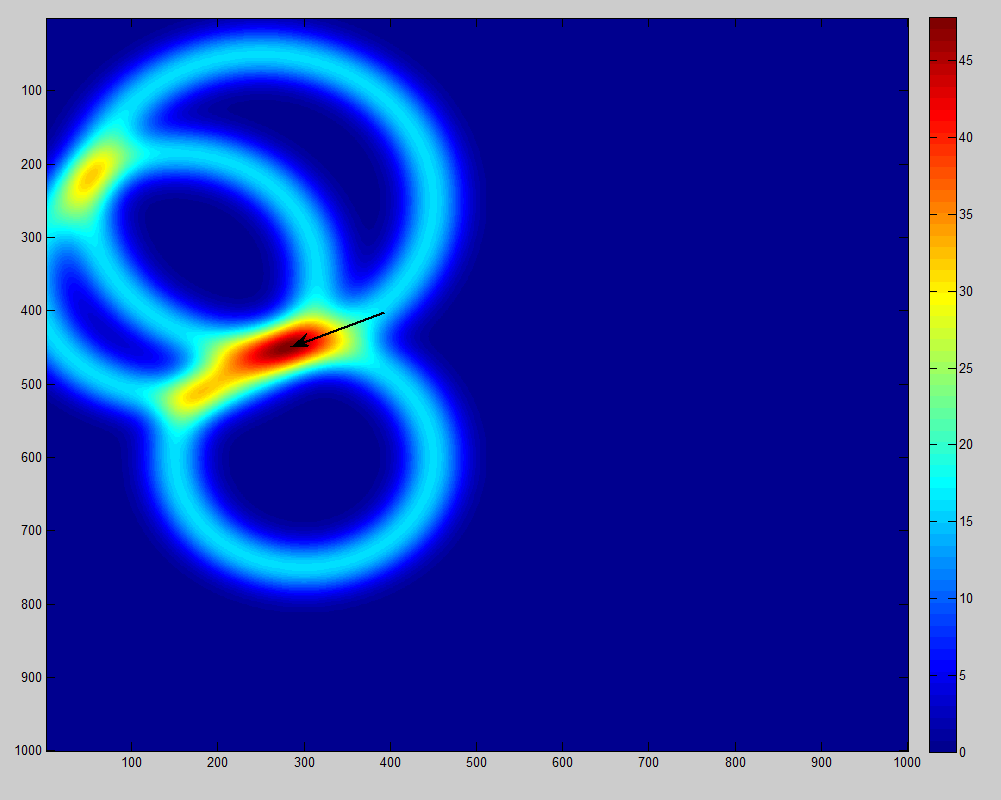
\includegraphics[width=0.75\textwidth]{guasianRouter}
\end{figure}
Zaprezentowany sposób wyznaczania lokalizacji dotyczył obliczeń w przestrzeni dwuwymiarowej. Przejście na przestrzeń trójwymiarową nie stanowi problemu - jedynymi zmianami, jakie należy wprowadzić, są:
\begin{itemize}
	\item wykonywanie obliczeń dla punktów $(X,Y,Z)$
	\item zmiana sposobu obliczania odległości euklidesowej między odbiornikiem, a transmiterem - należy wyznaczać odległość w przestrzeni trójwymiarowej.
\end{itemize}

\chapter{Propagacja sygnału radiowego}
\label{cha:teoria}
\section{Zanik sygnał radiowego}
Sygnał radiowy, wysłany przez urządzenie, w wyniku przechodzenia przez ośrodek (najczęściej jest nim powietrze) ulega zanikowi. Różnica w mocy sygnału odczytanego przez odbiornik, a siłą sygnału wysłanego przez nadawcę, pozwala na obliczenie odległości pomiędzy dwoma urządzeniami. Dodatkowymi współczynnikami, które mają wpływ na obliczenia, są:
\begin{itemize}
	\item zysk energetyczny anteny nadawcy oraz odbiorcy
	\item margines zaniku, który zależy od czułości odbiornika
	\item straty w sile sygnalu wynikające ze środowiska - przeszkody, odbicia, inne urządzenia nadające
\end{itemize}
\begin{figure}[H]			
	\centering
	\caption{Schemat zaniku sygnału}
	\includegraphics[width=0.75\textwidth]{zanik_sygnalu}
\end{figure}
\section{Zysk energetyczny anteny}
Zysk energetyczny anteny jest to stosunek mocy ateny wypromieniowanej w danym kierunku do mocy wypromieniowanej przez antenę wzorcową. Anteną wzorcową może być m.in. antena izotropowa, czyli antena bez fizycznych rozmiarów, która cały sygnał zasilany wysyła we wszystkich kierunkach. W takim wypadku, zysk energetyczny anteny wyrażany jest w $dBi$.\\
Na zysk energetyczny mają również wpływ kierunkowość oraz materiał, z którego wykonana jest antena.
\section{Margines zaniku}
Margines zaniku (fade margin) jest to wartość określająca wielkość "marginesu" pomiędzy wartością odebraną, a czułością odbiornika. Określa się ją wzorem:
\begin{equation}
FM = P_{rs} - P_{rx}
\end{equation}
gdzie $P_{rs}$ to siła odebranego sygnału.\\
Margines zaniku jest wyznacznikiem, jak "dobre" jest połączenie między transmiterem i odbiorcą. Czym wyższa wartość marginesu zaniku, tym bardziej niezawodne jest połączenie.
Wartość marginesu zaniku określa się w jednostce $dB$.
\section{Received signal strength indication}
Received signal strength indication (skrótem RSSI) jest to miara określająca moc sygnału odbieranego. Przyjmuje ona wartości niedodatnie (gdzie 0 oznacza sygnał najsilniejszy). Jednostką, w jakiej określa się siłę sygnału jest $dBm$, która jest logarytmiczną jednostką miary mocy odniesiona do mocy $1mW$.\\
System Android pozwala na odczytanie siły odbieranego sygnału. Można do tego wykorzystać API $WifiManager$ (w przypadku odczytu sygnału WiFi) oraz $BroadcastReceiver$ (w przypadku odczytu sygnału Bluetooth).
\section{Free-space path loss}		  		  
Utrata w sile sygnału spowodowana przejściem fali elektromagnetycznej przez ośrodek (najczęściej powietrze).
Wzór na obliczanie FSPL:
\begin{equation}
FSPL = P_{tx} + AG_{tx} + AG_{rx} - P_{rx} - FM - L
\end{equation}
%http://electronicdesign.com/communications/understanding-wireless-range-calculations
%Microwave and Millimetre-Wave Design for Wireless Communications  Autorzy Ian Robertson,Nutapong Somjit,Mitchai str 449
%https://en.wikipedia.org/wiki/Free-space_path_loss
%http://www.tplink.com/ie/support/calculator/#1
%http://stackoverflow.com/questions/11217674/how-to-calculate-distance-from-wifi-router-using-signal-strength
Gdzie symbole oznaczają:
\begin{itemize}
	\item $P_{tx}$ - siła trasmitera, wyrażona w dBm
	\item $AG_{tx}$ - zysk energentyczny anteny transmitera, wyrażony w dBi
	\item $AG_{rx}$ - zysk energentyczny anteny odbiorcy, wyrażony w dBi
	\item $P_{rx}$ - czułość odbiornika, wyrażona w dBm
	\item $FM$ - margines zaniku sygnału (fade margin) - określa jak duży jest margines różnicy pomiędzy uzyskaną siłą sygnału, a czułością odbiornika
	\item $L$ - straty wynikające np z oddziaływania innych transmiterów, przeszkód itp.
\end{itemize}
Dodatkowo, FSPL można obliczyć, używając następujący wzór:
\begin{equation}
FSPL = 20log_{10}\left(\frac{d}{d_{0}}\right) + 20log_{10}(f) + K
\end{equation}
%Indoor Localization Method Based on Wi-Fi Trilateration Technique Maxim Shchekotov
% Wi-Fi Indoor Positioning System Based on RSSI Measurements from Wi-Fi  Access Points  –  A Tri-lateration Approach Onkar Pathak, Pratik Palaskar, Rajesh Palkar, Mayur Tawari
Gdzie symbole oznaczają:
\begin{itemize}
	\item $d$ - dystans dzielący trasmiter od odbiorcy, wyrażony w metrach
	\item $d_{0}$ - dystans referencyjny -  w tym wypadku 1 metr
	\item $f$ - częstotliwość transmitera - wyrażona w MHz
	\item $K$ - stała, którą można określić wzorem:
	\begin{equation}
	K = 20log_{10}\left(\frac{4\pi d_{0}}{C}\right)
	\end{equation}
	gdzie $d_{0}$ to dystans referencyjny (taki sam jak we wzorze wyżej), a $C$ to długość fali emitowanej przez transmiter
\end{itemize}	  
Po przekształceniu wzoru, uzytkujemy:
\begin{equation}
d = 10^{\left(\frac{FSPL - K - 20log_{10}(f)}{20}\right)}
\end{equation}
A po połączeniu obu wzorów dostajemy:
\begin{equation}
d = 10^{\left(\frac{P_{tx} + AG_{tx} + AG_{rx} - P_{rx} - FM - L - K - 20log_{10}(f)}{20}\right)}
\end{equation}
Po podstawieniu wzoru na margines zaniku do wzoru (5), uzyskujemy
\begin{equation}
d = 10^{\left(\frac{P_{tx} + AG_{tx} + AG_{rx} - P_{rs} - L - K - 20log_{10}(f)}{20}\right)}
\end{equation}
\chapter{Testy sposobów komunikacji radiowej}
\label{cha:teoria}

Testy mają na celu zbadać skuteczność wyznaczania odległości między transmiterem, a odbiornikiem dla sygnałów Wifi i Bluetooth.\\
Testy odbywać się będą w dwóch etapach:
\begin{itemize}
	\item w pierwszym, odbiornik i transmiter będą oddalone od siebie o około 1m. Mierzona będzie siła odbieranego sygnału. Celem tego etapu jest określenie, jak duże straty siły sygnału związane są z komunikacją Wifi i Bluetooth. Straty mogą wynikać z izolacji obudowy, odbić, interferencji kilku fal lub z braku kierunkowości anteny (antena wbudowana).
	\item w drugim etapie, obliczone wcześniej wartości strat zostaną wykorzystane, aby zmierzyć, jak zmienia się siła sygnału, kiedy na drodze pojawi się przeszkoda. Do testów wykorzystana została książka o formacie A4 grubości 7 centymetrów, drewniane drzwi o grubości 5 centymetrów oraz ściana o grubości 26 centymetrów.
\end{itemize}
Uzyskane informacje pozwolą obliczyć współczynnik strat, jaki należy uwzględnić podczas późniejszego obliczania lokalizacji użytkowników oraz pozwoli przydzielić każdemu ze sposobów komunikacji radiowej odpowiednią wagę, w zależności od jego odporności na zakłócenia.
\section{Wykorzystane urządzenia}
\begin{enumerate}
	\item Smartphone Sony Xperia Z1 Compact (D5503) - odbiornik\\				
	Dane techniczne:
	\begin{itemize}
		\item Częstotliwość - 2,4GHz
		\item Przyrost siły sygnału z anteny WiFi - 2dBi
		\item Przyrost siły sygnału z anteny Bluetooth - 0dBi
	\end{itemize}
	\item Router TP-Link TD-W8970 - nadajnik\\
	Dane techniczne:
	\begin{itemize}
		\item Częstotliwość - 2,4GHz
		\item Dwie zewnętrzne anteny kierunkowe
		\item Przyrost siły sygnału z anteny - 4dBi
		\item Siła transmitera - 16.5dBm					
	\end{itemize}
	%\item Router TP-Link TL-WA701ND - nadajnik\\
	%Dane techniczne:
	%\begin{itemize}
	%	\item Częstotliwość - 2,4GHz
	%	\item Jedna zewnętrzna antena kierunkowa
	%	\item Przyrost siły sygnału z anteny - 2dBi
	%	\item Siła transmitera - 15dBm					
%	\end{itemize}
	\item Smartphone Samsung Grand 2 (G7102) - nadajnik\\
	Dane techniczne:
	\begin{itemize}
		\item Jedna antena wbudowana
		\item Przyrost siły sygnału z anteny - 0dBi
		\item Siła transmitera Bluetooth - 6dBm				
	\end{itemize}
\end{enumerate}
\section{Warunki}
Wszystkie pomiary wykonywane były w pomieszczeniu zamkniętym, bez przeszkód na drodze sygnału. Wszystkie urządzenia znajdowały się na tej samem wysokości, skierowane do siebie górną częścią obudowy (w przypadku routera, skierowany był on do odbiornika swoimi antenami kierunkowymi).
\begin{figure}[H]
	\centering			
	\caption{Zdjęcie urządzeń pomiarowych oraz środowiska testowego}
	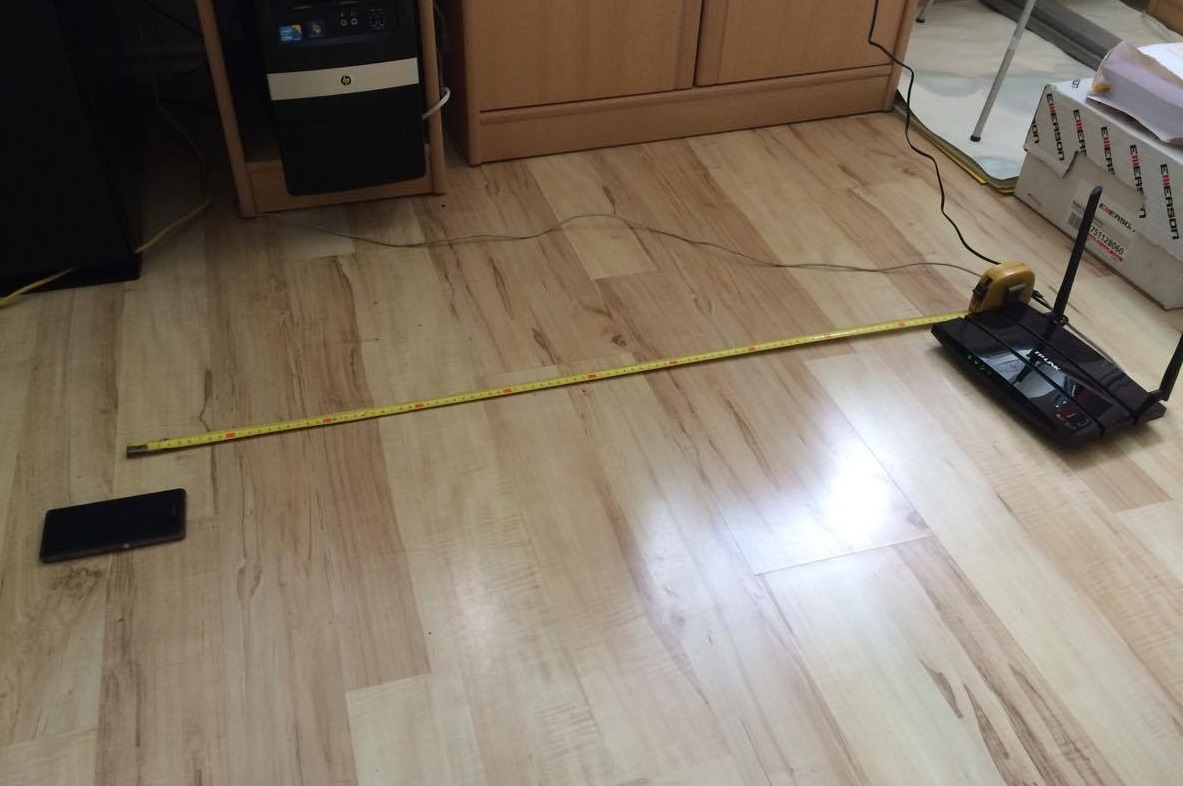
\includegraphics[width=0.75\textwidth]{srodowisko_pomiarowe}
\end{figure}
\section{Pobranie danych i analiza wyników}
Dla każdego eksperymentu została wykonana odpowiednio duża ilość powtórzeń (od 70 do 120), aby wynik był dokładniejszy. W tym celu, została stworzona lekka aplikacja, która pobierała zgłoszenia telefonu i zapisywała je do pliku tekstowego. Następnie, po skończonych testach, parsowała dane i wyliczała średnią dla sił sygnałów pochodzących z interesującego nas źródła (sygnały pochodzące z innych źródeł były odrzucane). Tak obliczone dane zostały zawarte w tabelach w dalszej części rozdziału.
\section{Wyznaczenie wartości strat}
Eksperyment polegał na ustawieniu transmitera w odległości 1 metra od odbiornika, na jednym poziomie, antenami do siebie. Na podstawie siły sygnałów obliczana została wartość strat, jakie musiałyby być uwzględnione, aby odległość obliczona równała się odległości fizycznej.\\			
\begin{figure}[H]
	\centering			
	\caption{Szkic eksperymentu nr 1}
	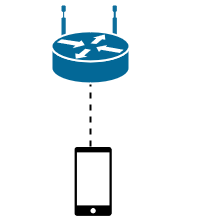
\includegraphics{exper1}
\end{figure}
\subsection{Pomiary}
	Wartości obliczone dla eksperymentu nr 1, w którym Router TP-Link TD-W8970 jest transmiterem sygnału Wifi, a Samsung Grand 2 transmiterem Bluetooth:
	\begin{center}
		\begin{minipage}{\linewidth}
			\begin{tabular}{|c|c|c|c|}
				\hline 
				Sygnał & Ilość prób & Średnia siła sygnału (w dBm) & Obliczona średnia wartość strat (dB) \\ 
				\hline 
				Wi-Fi & 163 & -38.88 & 21.18 \\ 
				\hline 
				Bluetooth & 113 & -57.5 & 23.3 \\ 
				\hline 
			\end{tabular} 
		\end{minipage} 
	\end{center}
\subsection{Wnioski}
Z danych uzyskanych podczas eksperymentu wynika, że straty spowodowane zakłóceniami sygnału Bluetooth są wyższe niż spowodowane zakłóceniami sygnału WiFi. Może się to wiązać z tym, że transmiter Wifi ma większą moc, zaś kierunkowe anteny zmniejszają ilość zakłóceń wynikających z odbicia się sygnału. Wartości strat obliczone dla obu sposobów komunikacji zostaną wykorzystane podczas eksperymentu nr 2 oraz będą miały wpływ na wybór wagi dla siły sygnałów podczas określania lokalizacji użytkowników.
\section{Przeszkody na drodze sygnału}
Drugi eksperyment ma na celu zbadanie odporności każdego z rodzajów sygnałów na zakłócenia związane ze stojącą na drodze przeszkodą. Wnioski z tego eksperymentu będą miały duży wpływ na działanie systemu, ponieważ w rzeczywistym środowisku, w którym ma działać tworzony system, transmiter od użytkownika będzie dzielić czasami nawet kilka ścian i ważne jest, aby odpowiednio dobrać wagi dla sygnałów.\\
W pierwszej części eksperymentu, transmiter został oddalony od odbiornika o 1 metr. Na drodze sygnału została postawiona gruba książka w formacie A4. W drugiej części eksperymentu, transmiter od odbiornika oddalony został o 2 metry, w taki sposób, aby na drodze sygnału znalazły się najpierw drewniane drzwi, a w kolejnej części eksperymentu ściana.\\
Do dokonania pomiarów zostały wykorzystane te same urządzenia jak w przypadku eksperymentu nr 1.\\
Wartość błędu bezwzględnego obliczana była na podstawie wzoru:
\begin{equation}
\delta = |D_r - D_o|
\end{equation}
gdzie $D_r$ to rzeczywista odległość między transmiterem, a odbiornikiem, zaś $D_o$ to odległość obliczona na podstawie siły sygnału.
\begin{figure}[H]
	\centering			
	\caption{Szkic eksperymentu nr 2}
	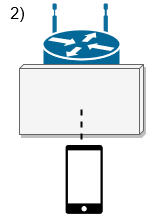
\includegraphics{exper2}
\end{figure}
\subsection{Pomiary}
Wartość siły sygnałów, obliczony dystans oraz wielkość błędu dla pomiaru sygnału Wifi i Bluetooth, dla którego przeszkodą była książka przy dystansie 1 metra:
\begin{center}
	\begin{minipage}{\linewidth}
		\begin{tabular}{|c|c|>{\centering} p{3cm}|>{\centering} p{3cm}|c|}
			\hline 
			Sygnał & Ilość pomiarów & Średnia siła sygnału (w dBm) & Średnia obliczona odległość (m) & Błąd bezwzględny (m)\\ 
			\hline 
			Wifi & 182 & -40,81 & 1,24 & 0,24 \\ 
			\hline 
			Bluetooth & 70 & -61.46 & 1,57 & 0,57 \\ 
			\hline 			
		\end{tabular} 
	\end{minipage} 
\end{center}
Wartość siły sygnałów, obliczony dystans oraz wielkość błędu dla pomiaru sygnału Wifi i Bluetooth, dla którego przeszkodą były drzwi przy dystansie 2 metrów:
\begin{center}
	\begin{minipage}{\linewidth}
		\begin{tabular}{|c|c|>{\centering} p{3cm}|>{\centering} p{3cm}|c|}
			\hline 
			Sygnał & Ilość pomiarów & Średnia siła sygnału (w dBm) & Średnia obliczona odległość (m) & Błąd bezwzględny (m)\\ 
			\hline 
			Wifi & 112 & -48,1 & 2,89 & 0,89 \\ 
			\hline 
			Bluetooth & 107 & -67,05 & 3,01 & 1,01 \\ 
			\hline 			
		\end{tabular} 
	\end{minipage} 
\end{center}
Wartość siły sygnałów, obliczony dystans oraz wielkość błędu dla pomiaru sygnału Wifi i Bluetooth, dla którego przeszkodą była ściana przy dystansie 2 metrów:
\begin{center}
	\begin{minipage}{\linewidth}
		\begin{tabular}{|c|c|>{\centering} p{3cm}|>{\centering} p{3cm}|c|}
			\hline 
			Sygnał & Ilość pomiarów & Średnia siła sygnału (w dBm) & Średnia obliczona odległość (m) & Błąd bezwzględny (m)\\ 
			\hline 
			Wifi & 103 & -48,3 & 2,96 & 0,96 \\ 
			\hline 
			Bluetooth & 110 & -66,95 & 2,97 & 0,97 \\ 
			\hline 			
		\end{tabular} 
	\end{minipage} 
\end{center}
\subsection{Wnioski}
Wyniki eksperymentu nr 2 jasno wskazują, że sygnał Wifi jest bardziej odporny na zmiany spowodowane pojawiającą się na drodze przeszkodą. Ma to duży wpływ na obliczanie lokalizacji użytkownika na podstawie sygnału i dlatego technologia Wifi będzie miała wyższą wagę w tworzonym systemie.\\
Dodatkowo, warto zwrócić uwagę, że błędy wynikające z obecności na drodze sygnału drzwi oraz ściany są mniejsze, niż można się było spodziewać. Może to wynikać z faktu, że sygnał nie rozchodzi się tylko w jednym kierunku i dzięki temu, podczas przechodzenia przez drzwi, część sygnału napotykała również na ścianę, co spowodowało większe zakłócenia.
\chapter{Implementacja}
\label{cha:implementacja}
\section{Architektura}
Archtektura systemu oparta jest na topologii gwiazdy. Centralny punkt stanowi serwer, z którym łączą się aplikacje mobilne, odpowiedzialne za lokalizację użytkowników, którzy z nich korzystają. Telefony komunikują się z serwerem jednostronnie, a jedyną zwrotną informacją, jaką uzyskują, jest to, czy żądzanie zostało pozytywnie przyjęte.\\
Do serwera mogą podłączać się również aplikacje klienckie, pozwalające administratorom na konfigurację oraz podgląd zebranych przez serwer lokalizacji. Podstawowym warunkiem komunikacji między serwerem, a użytkownikiem aplikacji klienckiej jest wcześniejsza autoryzacja loginem i hasłem.\\
Aplikacja serwerowa połączona jest z bazą danych, w której przechowywane są lokalizacje użytkowników oraz dane konfiguracyjne systemu. W architekturze wykorzystana jest open-sourcowa baza danych PostgreSQL. Dostęp do danych zapewniony jest przy użyciu mapowania obiektowo-relacyjnego, zaś wykorzystanie wzorca projektowego 'Repozytorium' pozwala na odseparowanie warstwy logiki biznesowej aplikacji od warstwy danych. Dostęp aplikacji klienckich do danych może się odbywać tylko i wyłącznie przy pośrednictwie aplikacji serwerowej.\\
Ostatnim elementem, z którym komunikuje się serwer, są urządzenia sterowane. Fizycznie nie należą do systemu, ponieważ nie są dostarczane oraz z góry zdefiniowane podczas wdrażania systemu. Są jednak podstawowym elementem, dzięki któremu system ma sens działania. Urządzenia sterujące to wszystkie urządzenia, które są zdefiniowane w aplikacji serwerowej, a którymi steruje serwer. Serwer zarządza urządzeniami na podstawie lokalizacji użytkowników. Medium komunikacji nie jest z góry narzucone - w zaimplementowanym domyślnie module komunikacyjnym, wysyłanie informacji pomiędzy serwerem, a urządzeniami odbywa się przy użyciu protokołu HTTP.
\begin{figure}[H]			
	\centering
	\caption{Schemat architektury systemu}
	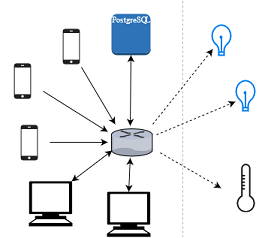
\includegraphics{schemat_architektury}
\end{figure}
\section{Wykorzystana technologia}
Podstawową i główną technologią wykorzystaną podczas tworzenia systemu jest .NET Framework. Jest to stworzona przez firmę Microsoft platforma programistyczna, która pozwala na tworzenie efektownych, nowoczesnych aplikacji. Podstawowym językiem, w którym napisane są wszystkie aplikacje należące do systemu, jest C\#. Jest to obiektowy język programowania, jeden z najważniejszych języków wykorzystywanych podczas tworzenia aplikacji na platformę .NET.\\
Aplikacja serwerowa wykorzystuje serwisy udostępniane przez ASP.NET. Jest to webowa platforma, wchodząca w skład .NET Framework, która pozwala na tworzenie aplikacji opartych na architekturze Model-View-Controller. Komunikacja serwera z aplikacjami odbywa się przy użyciu protokołu HTTP. Platforma ASP.NET wspiera wykorzystanie czasowników HTTP, a w połączeniu z zastosowaniem stylu architektonicznego REST, pozwala na wydajną i efektowną współpracę wszystkich elementów systemu - aplikacji mobilnej i klienckiej.\\
Algorytm określania lokalizacji użytkownika oraz wzory obliczające dystans dzielący aplikację mobilną od routerów i Beaconów zostały napisane w F\#. Jest wieloparadygmatowy, głównie funkcyjny, język programowania, wspierany przez platformę .NET. Wybrałem ten język do wypisanych powyżej zadań, ponieważ uważam, że języki funkcyjne najlepiej nadają się do algorytmów opartych na wzorach matematycznych - w przeciwieństwie do innych języków, zachowują czystość i czytelność kodu, nie tracąc nic na szybkości wykonywania. Dodatkowo, zależało mi na poznaniu i nauczeniu się podstaw pisania w tym języku. Algorytmy lokalizacji napisane są w osobnym projekcie, a dzięki skompilowaniu kodu do przenośnej biblioteki .NET, mogą być bezproblemowo podłączone do aplikacji serwerowej.\\
Serwer, podczas dostępu do danych, wykorzystuje biblitekę NHibernate. Jest to narzędzie do mapowania obiektowo-relacyjnego, które pozwala na szybki dostęp oraz operowanie na danych zapisanych w bazie danych. Połączenie serwera z bazą zarządzane jest przez narzędzie NpgSQL - dostawcę danych, korzystającego z bibliotek ADO.NET.\\
Systemem, na który stworzona jest aplikacja mobilna, jest Android. Aplikacja jest również tworzona w języku C\#, na co pozwala wykorzystanie frameworka Xamarin. Xamarin pozwala na pisanie aplikacji w języku C\# na wszystkie najpopularniejsze platformy. Jest to najważniejszy powód, dla którego wybrałem ten framework jako główne narzędzie do tworzenia swoje aplikacji mobilnej. Takie podejście pozwoli mi w przyszłości, w ramach potrzeby, na szybsze przejście na inne platformy mobilne. Kod napisany w Xamarinie jest tłumaczony w momencie kompilacji na kod zarządzany natywnego języka platformy Android, Javę, przez co nie powoduje on spadku wydajności aplikacji. Dodatkowym powodem, dla którego sięgnąłem po to narzędzie, była chęć nauczenia się korzystania z niego.\\
Aplikacje klienckie korzystają z WinForms - biblioteki klas GUI, wchodzące w skład .NET Framework. Aplikacja wymaga, aby na komputerze osoby korzystające z niej zainstalowany był .NET Framework w wersji 4.5 albo wyższej.
\section{Konfiguracja}
Aplikacja serwerowa jest dostarczona jako Web Deployment Package, który należy wdrożyć do stworzonej wcześniej witryny w menedżerze internetowych usług informacyjnych (IIS). Kiedy aplikacja zostanie poprawnie wdrożona, należy skonfigurować dane dostępowe do bazy danych poprzez edycję 'connection-string' w pliku Web.config w folderze serwera. Po tej operacji należy zrestartować serwer.\\
Aby utworzyć wymagane przez serwer struktury bazodanowe, należy wywołać w utworzonej dla systemu bazie danych skrypt SQL. Znajduje się on w pliku 'script.sql' i dostarczony jest on wraz plikiem wdrożeniowym serwera.\\
Przed uruchomieniem aplikacji administracyjnej, należy skonfigurować dane znajdujące się w pliku 'config.xml'. W danej 'PictureLocation' należy podać względną ścieżkę do mapy, odnosząc się do folderu, w którym znajduje się wykonywalna aplikacja. Do danej 'ServerIp' należy przypisać adres Ip serwera wraz z portem, zaś w ClientIp należy wstawić adres Ip klienta, bez portu. Dane 'Login' i 'Password' są opcjonalne i zawierają zapamiętane dane logowania, którymi wypełniane jest pierwsze okno aplikacji. Po włączeniu aplikacji i zalogowaniu się (domyślne dane logowania to 'admin' i 'admin'), okno konfiguracji pozwala na bardziej rozbudowaną konfigurację systemu.
\section{Serwer}
Serwer jest aplikacją, która ma analizować zabrane dane, sterować urządzeniami zewnętrznymi oraz stanowić most pomiędzy klientem administracyjnym, a aplikacjami mobilnymi. Na zadania aplikacji serwerowej składają się:
\begin{itemize}
	\item Zbieranie danych z aplikacji mobilnych oraz wyznaczanie lokalizacji użytkowników
	\item Zezwalanie użytkownikowi administracyjnemu na konfigurację systemu poprzez żądania aplikacji klienckiej
	\item Sterowanie i zarządzanie urządzeniami zewnętrznymi poprzez analizowanie danych odebranych z aplikacji mobilnych
	\item Dostarczanie, w formie skumulowanej lub w czasie rzeczywistym, danych na temat położenia użytkowników do analizy i monitoringu
\end{itemize}
\subsection{Lokalizacja użytkowników mobilnych}
\subsubsection{Pobranie i analiza danych}
Serwer pobiera dane od użytkowników w formie requestów HTTP. Każde żądanie wysłane na serwer musi posiadać adres MAC urządzenia Bluetooth wysyłającego oraz listę zarejestrowanych sygnałów. Każda pozycja na liście sygnałów musi posiadać nazwę urządzenia, którego sygnał został odebrany (w przypadku sygnału wysłanego przez router jest to SSID sieci, zaś w przypadku urządzeń Bluetooth jest to adres MAC), typ sygnału (WIFI albo Bluetooth) oraz zarejestrowaną siłę sygnału, określoną w dBm. \\
Następnie, dla każdego elementu z listy dociągane są stałe dane zarejestrowane w systemie - lokalizacja oraz waga sygnału. Dane na temat routerów oraz stałych urządzeń Bluetooth (np. Beconów) pobierane są z bazy danych. Jeżeli jakiś sygnał Bluetooth nie widnieje w bazie danych, sprawdzane są ostatnie żądania od urządzeń mobilnych, dla których udało się określić lokalizację, a czas od ich ostatniej aktualizacji nie jest większy od 4 sekund. Jeżeli sygnał pochodzi od jednego z tych urządzeń, potrzebne informacje pobierane są z dynamicznie budowanej, lokalnej bazy wiedzy. Jeżeli sygnał nie figuruje ani w bazie danych, ani w bazie dynamicznej, zostaje uznany jako sygnał przypadkowy i odrzucony. Waga sygnału przyjmuje wartości w skali od 1 do 4. Domyślnie, sygnałowi pochodzącemu od routera WiFi nadawana jest waga 3, sygnałowi ze stałego urządzenia Bluetooth waga 2, zaś sygnały pochodzące od innych użytkowników mobilnych mają wagę 1. Wagę stałych urządzeń WiFi i Bluetooth można edytowac przy użyciu panelu konfiguracyjnego w aplikacji klienckiej. W ostatnim kroku, dla każdego zarejestrowanego sygnału obliczana jest odległość urządzenia od użytkownika. Wykorzystywana do tego jest lokalizacja użytkownika, wzór na Free-space path loss oraz dane statyczne (jak siła anten, siła trasmitera itp.).\\
\subsubsection{Algorytmiczne wyznaczenie lokalizacji}
Celem algorytmu jest wyznaczenie punktu, dla którego suma prawdopodobieństw wynikających z odległości użytkownika od urządzenia, jest największa.\\
Dane pobrane od użytkownika, uzupełnione o statyczne dane przechowywane w systemie, przekazane są do sekcji napisanej w języku F\#. Na wstępie, do każdego zarejestrownego sygnału zostaje przypisana funkcja probabilistyczna Guassa, określająca prawdopodobieństwo znalezienia się użytkownika w danym punkcie w przestrzeni, gdzie stała $\mu$ przyjmuje wartość równą dystansowi obliczonemu na podstawie siły sygnału urządzenia. Dzięki takiemu podejściu, każdy sygnał można zwizualizować jako sferę, której powierzchnia zbliżona jest do chmury. Największe zagęszczenie prawdopodobieństwa występuję dla średnicy równej odległości obliczonej z siły sygnału, rzednie zaś zbliżając się i oddalając od środka sfery.\\
Pierwszym krokiem algorytmu jest wyznaczenie prostapadłościanu, dla którego wykonywane będą obliczenia. Wielkość bryły dobrana jest tak, aby wewnątrz niej znalazły się wszystkie sfery sygnałów (przy uwzględniu zapasu równego 2$\sigma$). Następnie prostopadłościan oraz sfery są normalizowane w taki sposób, aby początek układu zaczył się w punkcie (0,0,0), zaś wszystkie wartości współrzędnych przyjmowały tylko wartości nieujemne. Celem takiej operacji jest uproszczenie algorytmu oraz usunięcie potrzeby skalowania iteratorów oraz odnośników do elementów w tablicach.\\
Kolejnym krokiem algorytmu jest podział prostopadłościanu na części, dla których liczona będzie suma prawdopodobieństw. Celem tego kroku jest podział pola działania na jednakowe sześciany w taki sposób, aby w żadnym wymiarze ilość sześcianów nie przekroczyła 100. Aby to uzyskać, najdłuższy bok prostopadłościanu zostaje podzielony na 100 częście. Następnie, boki w pozostałych 2 wymiarach zostają podzielone na sześciany o krawędziach o równej długości. Podział prostopadłościanu na sześciany pozwala na wyeliminowanie błędów obliczeniowych wynikających z nierealistycznego podziału pola obliczeniowego.\\
Kolejnym krokiem algorymtu jest wyliczenie sumy prawdopodobieńst ze wszystkich sfer sygnałów dla każdego sześcianu w prostopadłościanie. Każde prawdopodobieństwo, będące składową sumy, przemnażane jest przez wagę danego sygnału.		
\begin{equation}
P(x,y,z) = \sum_{r=1}^{r=R} w_r * \frac{1}{\sigma\sqrt{2\pi}}e^{\left(\frac{-(d-\mu)^2}{2\sigma^2}\right)}
\end{equation}
gdzie:
\begin{itemize}
	\item x, y, z - współrzędne konkretnego sześcianu
	\item R - ilość routerów w modelu
	\item $w_r$ - waga konkretnego routeru
	\item $\sigma$ - odchylenie standardowe, w naszym modelu wynosi: długość najdłuższego boku prostopadłościanu podzielona przez 30
	\item $\mu$ - średnia, w naszym modelu jest to wartość równa, obliczonej na podstawie siły sygnału, odległości użytkownika od źródła sygnału
	\item d - odległość Euklidesowa pomiędzy sześcianem, a routerem
\end{itemize}
Następnie wybierany jest sześcian, dla którego suma prawdopodobieństwa jest najwyższa. Jeżeli długość boku sześcianu jest równa lub mniejsza od naszego przybliżenia, współrzędna sześcianu staje się lokalizacją naszego użytkownika. Jeżeli długość boku sześcianu jest większa, dla wybranego sześcianu dobierane są jego sześciany sąsiednie. Następnie wybrane 27 sześcianów staje się nowym modelem obliczeniowym. Każdy wymiar nowego pola dzialony jest na 9 równych części, dzięki czemu uzyskuje się 729 sześcianów. Algorytm zostaje powtórzony, aż lokalizacja nie zostanie określona z interesującym nas przybliżeniem. Sześcian o największej sumie prawdopodobieństw staje się lokalizacją użytkownika.\\
Ostatnim krokiem algorytmu jest przeliczenie obliczonej lokalizacji przy użyciu danych uzyskanych podczas normalizacji, aby obliczone współrzędne odpowiadały lokalizacji dla danych wejściowych.
\subsubsection{Zarządzanie lokalizacją użytkownika}
Po pozytywnym obliczeniu lokalizacji, zostaje ona zapisana w bazie danych, aby potem mogła być użyta do wyświetlenia skumulowanej mapy przepływu użytkowników albo do sterowania urządzeniami. Następnie, lokalizacja zostaje asynchronicznie wysłana do wszystkich klientów administracyjnych, którzy zarejestrowali swoją chęć pobierania danych w trybie real-time (w czasie rzeczywistym). Lokalizacja wraz z adresem MAC użytkownika zostaje przekazana do wątków urządzeń sterowanych, które wykorzystują te dane do podjęcia decyzji o wywołaniu przypisanego urządzeniowi eventu. W ostatnim kroku, lokalizacja zostaje dodana (lub podmieniona, jeżeli wpis o danym użytkowniku już istnieje) w bazie dynamicznej, aby ta informacja mogła posłużyć przy wyznaczaniu lokalizacji innych użytkowników.
\subsection{Sterowanie i zarządzanie urządzeniami}
Serwer, poza pobieraniem i analizą danych, zajmuje się również sterowaniem przydzielonymi mu urządzeniami. Sterowanie urządzeniami odbywa się na dwa sposoby:
\begin{itemize}
	\item Przy użyciu eventów - urządzenia mogą mieć przypisaną klasę obsługującą zdarzenia specjalne. Mechanizm analizuje w czasie rzeczywistym ostatnie zarejestrowane lokalizacje użytkowników, a następnie na ich podstawie oraz na podstawie wcześniej przypisanych sobie reguł, decyduje, czy mają zostać podjętę jakieś działania. Jeżeli tak, komunikuje się z urządzeniem, aby ustawić mu wyznaczone parametry. Wywołana metoda zwraca zmienną typu Boolean, określającą, czy została podjęta decyzja o komunikacji z urządzeniem.
	\item Co określony interwał czasowy - mechanizm, który co jakiś określony czas oblicza parametry, jakie należy przekazać do urządzenia. Robi to na podstawie zarejestrowanych przez ten czas pozycji użytkowników. Do swoich obliczeń wykorzystuje wagi użytkowników, przypisane im w panelu administracyjnym. Mechanizm czasowy ma niższy priorytet niż mechanizm eventów, dlatego jeżeli klasa obsługująca zdarzenia przekazała urządzeniu parametry, system czasowy zostaje zawieszony aż do kolejnego przejścia pętli. Takie rozwiązanie zapobiega nadpisywaniu parametrów wysłanych do urządzenia, zanim wcześniejsze zostaną wykorzystane.
\end{itemize}
Informacje na temat urządzeń przechowywane są w bazie danych. Danymi, które są potrzebne do sterowania urządzeniem, niezależnie od jego typu, są:
\begin{itemize}
	\item jego lokalizacja (określona przez 3 współrzędne)
	\item adres ip urządzenia oraz port, na którym nasłuchuje
	\item nazwa rozpoznawalna przez użytkownika (np żarówka na korytarzu)
	\item sterownik określający sposób komunikacji, implementujący interfejs przypisany do konkretnego typu urządzenia
	\item informacja o przypisanym do urządzenia module sterowania eventami (np natychmiastowa zmiana siły oświetlenia, spowodowana zbliżeniem się określonego użytkownika)
	\item flaga określająca, czy dane urządzenie jest aktywne
\end{itemize}
\subsubsection{Dobór parametrów sterujących}
Dla każdego aktywnego urządzenia zapisanego w systemie, uruchomiony jest na serwerze osobny wątek sterujący. Taki sposób pracy został przyjęty, aby sterowanie i obsługa eventów odbywała się płynnie i w równy sposób dla wszystkich urządzeń, a błąd czy problemy komunikacyjne jednego z urządzeń nie miały wpływu na inne. Do każdego wątku sterującego przypisany jest obiekt klasy zawierającej wszystkie potrzebne informacje oraz metody, aby kontrolować dany typ urządzenia (dla oświetlenia jest to klasa LightDeviceControllingThread).\\
Praca wątku polega na wywołaniu metody StartControll(), na której ciało słada się nieskończona pętla while. Niezależnie od typu urządzenia, którym zarządza wątek, każda klasa posiada obiekt kolejki, do której kontroler przyjmujący dane od urządzeń mobilnych wstawia obliczone lokalizacje (pod warunkiem, że dla urządzenia sterowanego przypisano klasę obsługującą zdarzenia).\\
Kolejnym krokiem, jaki wykonywany jest w metodzie, jest pobranie z kolejki wszystkich oczekujących lokalizacji, a następnie przekazanie ich do klasy sterującej eventami. W systemie zaimplementowana jest przykładowa klasa sterująca światłem - ImportantUserFirstContr. Wybiera z listy tych użytkowników, którzy są w bliskiej odległości od źródła światła, a następnie wyszukuje wsród nich użytkowników o najwyższej wadze. Jeżeli taki użytkownik zostanie znaleziony, system wysyła do urządzenia rozkaz ustawienia światła o największej mocy. Taki poziom zostanie utrzymany aż ostatni użytkownik uprzywilejowany nie oddali się od źródła światła. System poczeka wtedy dodatkowe 4 sekundy, a następnie wyśle do urządzania informację o ustawieniu mocy światła na poprzednią wartość. System pozwala na rozszerzanie klas sterujących oraz tworzenie swoich i przypisywanie ich do urządzeń (o ile odpowiedni wpis zostanie dodany do bazy danych).\\
Jeżeli moduł zarządzania eventami zadecyduje o nie wysłaniu do urządzenia parametrów sterujących, wykonywany jest moduł zarządzania czasowego. Przed wykonaniem obliczeń, algorytm sprawdza, czy od ostatniej czasowej aktualizacji minął odpowiedni okres czasu (domyslnie algorytm ma się wykonywać co godzinę). Data poprzedniej aktualizacji przechowywana jest w polu LastUpdate, które jest aktualizowane obecną datą za każdym razem, gdy algorytm pozytywnie wyliczy parametry dla urządzenia. Jeżeli odpowieni czas minął, program pobiera z bazy wszystkie pozycje użytkowników, które zostały zarejestrowane w okresie od ostatniej aktualizacji. Następnie, algorytm wybiera z pobranej listy użytkowników, którzy zostali zarejestrowani w odległości nie większej niż, domyślne, 5 metrów, a następnie sumuje ich wagi. Parametr, jaki ma zostać wysłany do urządzenia jest liczony na podstawie wzoru:
\begin{equation}
P_{ustalona} = (P_{max} - P_{min}) * \frac{N_{blisk}}{N_{ogół}} + P_{min}
\end{equation}
gdzie zmienne w równaniu oznaczają:
\begin{itemize}
	\item $P_{ustalona}$ - moc światła jaka ma być ustawiona dla urządzenia
	\item $P_{min}$ - minimalna moc światła ustawiona dla urządzenia
	\item $P_{max}$ - maksymalna moc światła ustawiona dla urządzenia
	\item $N_{blisk}$ - suma wag użytkowników, którzy zostali zarejestrowani wystarczająco blisko urządzenia
	\item $N_{ogół}$ - suma wag wszystkich użytkowników w danym okresie czasowym
\end{itemize}
Wysyłany parametr jest ustawiany dodatkowo w zmiennej PreviousStaticPowerLevel, aby mógł być potem, w ramach potrzeby, wykorzystany przez moduł sterujący eventami. Na końcu, do zmiennej przechowywującej ostatnią aktualizacje zostaje przypisana obecna data i godzina.\\
Jeżeli parametry urządzenia zostały zaktualizone w obecnym przebiegu algorytmu, ponowne wykonywanie algorytmu rozpoczyna się od razu. Jeżeli nie, wątek zostaje uśpiony na 0,1 sekundy, aby nie zużywać niepotrzebnie zasobów serwera.
\subsubsection{Komunikacja z urządzeniami}
Sposób komunikacji serwera z urządzeniem nie jest zapisany bezpośrednio w kodzie serwera, ale jest przechowywany w bazie danych i przypisywany indywidualnie do konretnego urządzenia. Może zostać zmieniony przy użyciu panelu administracyjnego. Dla każdego typu urządzenia może być zdefiniowana pewna pula modułów komunikacji z urządzeniami. Każdy typ ma określony interfejs, po którym ma dziedziczyć klasa komunikująca się z tego typu urządzeniami. Wewnątrz modułu komunikacyjnego określony jest format wysyłanej wiadomości, kodowanie oraz kolejność parametrów. Ilość metod, które ma udostępniać klasa implementująca interfejs jest zależna od ilości parametrów, jakie mogą być ustawiane w danym typie urządzeń.
\begin{figure}[H]			
	\centering
	\caption{Model komunikacji z urządzeniami oświetleniowymi}
	\includegraphics[width=1.0\textwidth]{modul_komunikacji}
\end{figure}
W systemie został stworzony intefejs ILightDeviceInterface. Powinien być implementowany przez moduły do komunikacyjni z urządzeniami odpowiedzialnymi za oświetlenie. Z racji tego, iż światło posiada tylko jeden sterowalny parametr - moc światła, interfejs narzuca na klasie zaimplementowanie metody NotifyInformationToDevice, która jako parametry przyjmuje ip urządzenia, jego port oraz wartość mocy światła, jaka ma być wysłana do urządzenia. Zadaniem implementacji tej metody jest sformatowanie wiadomości, zawierającej ustawianą moc światła, według standardu urządzenia oraz wysłanie jej protokołem obslugiwanym przez urządzenie. Metoda ma zwrócić zmienną typu Boolean, informującą o tym, czy komunikacja i wysłanie wiadomości się powiodły.\\		
W ramach przykładu, stworzony został moduł do komunikacji z urządzeniami oświetleniowymi, LoggerLightDeviceInterface. Wysyła on protokołem HTTP na podany adres Ip wiadomość o formacie \textit{'Należy ustawić wartość na: $P_{swiatla}$'}, gdzie $P_{swiatla}$ to moc światła, którą chcemy ustawić.
\subsection{Konfiguracja systemu}
Aplikacja serwerowa pozwala na konfigurację elementów systemu bez potrzeby jego restartowania. Serwer wykorzystuje do tego kontroler ConfController, przyjmujący żądania HTTP. Podstawowymi elementami, które mogą być konfigurowane w taki sposób są:
\begin{itemize}
	\item wielkość pola operacyjnego - wartość określająca, jak duży jest obszar, na którym zainstalowany jest system. Wewnątrz tego pola muszą znajdować się wszystkie obsługiwane routery i urządzenia Bluetooth, ktore nie zmieniają swojej pozycji (np Beacony). Jednostką, w jakiej zapisana jest wielkość mapy, są metry. Wartość ta wykorzystywana jest podczas wyświetlania lokalizacji użytkowników w aplikacji administracyjnej - współrzędna lokalizacji zostaje przeskalowana przy użyciu wielkości pola w taki sposób, aby realistycznie odzorowywała położenie na wyświetlanej mapie.
	\item dane o routerach Wifi i nieporuszających się urządzeniach Bluetooth - administrator systemu ma możliwość zmiany kluczowych danych na temat urządzeń, na podstawie których lokalizowani są potem użytkownicy. Poza danymi technicznymi, dotyczącymi specyfikacji urządzenia (siła trasmitera, siła anten, straty wynikające z kształtu obudowy - np antena wewnętrzna), zdefiniowane są również:
	\begin{itemize}
		\item typ sygnału wysyłanego przez urządzenie - Wifi albo Bluetooth
		\item nazwa, po której urządzenie jest rozpoznawalne przez aplikację mobilną - SSID w przypadku routera WiFi, Mac w przypadku urządzenia Bluetooth
		\item lokalizacja urządzenia - wymagane jest podanie lokalizacji w trzech wymiarach. Współrzędne urządzenia, jak wszystkie współrzędne w systemie, są podawane stosunku do punktu określonego jako początek pola działania systemu.
		\item waga urządzenia, która uwzględniana jest podczas lokalizowania użytkownika. Wartość ta podczas dodawania nowego urządzenia, inicjalizowana jest wartościami domyślnymi, które potem można zmienić. Dopuszczalna wartość wagi jest liczbą całkowitą z zakresu $<1:4>$. Domyślne wartości to:
		\begin{itemize}
			\item dla urządzeń Bluetooth, dynamicznie zmieniających swoją pozycję (użytkownicy aplikacji mobilnej) - 1
			\item dla urządzeń Bluetooth, których lokalizacja jest określona - 2
			\item dla urządzeń Wifi - 3
		\end{itemize}
	\end{itemize}
	Dane na temat routerów przechowywane są w bazie danych, skąd są pobierane podczas startu aplikacji serwerowej. Informacje te są również przechowywane lokalnie, w pamięci serwera. Ma to na celu zmiejszenie czasu wykonywania operacji, ponieważ pobieranie danych z bazy danych jest dużo wolniejsze niż korzystanie ze zmiennych zapisanych w pamięci. Dlatego, każdorazowa zmiana informacji o routerach powoduje zmianę danych przechowywanych lokalnie przez serwer. System zakłada, że zmiany w danych o routerach dokonywane są tylko przy użyciu aplikacji serwerowej - zmiany dokonane na bazie przez zewnętrzne aplikacje (np GUI bazy danych) nie zostaną uwzględnione przez serwer aż do jego restartu.
	\item Dane na temat urządzeń sterowanych - podobnie jak w przypadku urządzeń do lokalizacji użytkowników, sterowane urządzenia mogą być dodawane, edytowane oraz usuwane przez administratorów systemu. Informacje różnią się w zależności od kategorii, do której należy dane urządzenie, jednak część z nich jest wspólna:
	\begin{itemize}
		\item nazwa - nazwa urządzenia, która ma pozwolić na jego identyfikację przez użytkowników systemu
		\item ip i port - podstawowe dane wykorzystywane do komunikacji z urządzeniem
		\item lokalizacja - położenie urządzenia określone przez trzy współrzędne
		\item moduł eventów - nazwa modułu, który ma obsługiwać wydarzenia związane z danym urządzeniem. Do urządzenia może nie być przypisany żaden moduł eventów
		\item moduł komunikacyjny - nazwa modułu, który ma pozwolić na komunikację serwera z urządzeniem
		\item czy moduł jest aktywny - informacja ta jest wykorzystywana podczas sterowania urządzeniem 
	\end{itemize}
	Informacje na temat sterowanych urządzeń, poza wpisami w bazie danych, przechowywane są również w pamięci serwera. W przeciwieństwie do routerów (których dane przechowywane są statycznie w klasie SystemDataKnowledge), dane na temat urządzeń znajdują się w przypisanych im obiektach sterujących. Jest to związane z tym, że wątki sterujące są jedynymi elementami aplikacji serwerowej, które często korzystają z tej informacji.\\
	Z racji tego, iż z każdym sterowanym urządzeniem, zarządzanym przez system, związany jest obiekt sterujący, kontroler konfigurujący odpowiedzialny jest również za edycję wątków sterujących. W przypadku dodawania do systemu nowego sterowanego urządzenia, kontroler inicjalizuje nowy obiekt sterujący oraz startuje związany z nim wątek. W przypadku usuwanie urządzenia, kontroler zatrzymuje wątek sterujący i usuwa jego obiekt z listy obiektów sterujących.
	\item Dane na temat użytkowników systemu - kontroler konfiguracyjny pozwala na edycję wagi użytkownika oraz jego nazwy. System rozpoznaje użytkowników po adresie MAC - zmiana nazwy użytkownika ma na celu jedynie pomóc osobie korzystającej z systemu łatwiejsze rozpoznawanie użytkowników. Waga używana jest przy sterowaniu urządzeniami - użytkownik o wadze 4 (przykładowo szef) jest ważniejszy z punktu widzenia modułu określającego parametry urządzeń, niż osoba o wadze 1 (zwykły pracownik). Dodatkowo, waga może mieć wpływ na moduły obsługi zdarzeń, przypisane do urządzenia - natężenie światła może uzyskiwać wartość maksymalną w przypadku pojawienia się w okolicy użytkownika o wadze 4.\\
	Dane o użytkownikach przechowywane są w bazie - nie ma potrzeby tworzyć lokalną kopię.
\end{itemize}
\subsection{Zarządzanie pozostałymi funkcjami aplikacji administracyjnej}
Do obsługi pozostałych, poza konfiguracją, żądań aplikacji klienckiej, służy kontroler ClientController. Zawiera on metody pozwalające na:
\begin{itemize}
	\item logowanie i wylogowywanie się użytkownika - użytkownik w momencie włączania aplikacji zmuszony jest do zalogowania się. Na serwer zostaje wysłane żądanie zawierające jego login. Następnie wysłany login zostaje powiązany z adresem ip, z którego przyszło żądanie. Jest to robione w celu umożliwienia późniejszego wysyłania informacji do klienta - wykorzystywane w momencie, w którym użytkownik zadeklaruje chęć monitorowania użytkowników mobilnych.
	\item pobranie informacji o sterowanych urządzeniach zarejestrowanych w systemie - lista urządzeń jest pobierana w celu wyświetlenia na mapie. Dodatkowo, pobierane są wszystkie przyrządy bez względu na ich kategorię. Zwracanymi informacjami są lokalizacja urządzenia (w celu wyświetlenia w odpowiednim miejscu) oraz jego kategoria (aby aplikacja kliencka mogła dobrać odpowiednią ikonkę).
	\item zgłoszenie żądania zapisania użytkownika do subskrypcji lokalizacji użytkowników - system zostaje poinformowany, że dany administrator chce monitorować wszystkich pojawiających się użytkowników aplikacji mobilnej. W momencie określenia lokalizacji użytkownika, do wszystkich użytkowników, na adres ip pobrany podczas logowania, zostaje wysłana notyfikacja zawierająca współrzędne użytkownika oraz jego adres MAC.
	\item pobranie lokalizacji użytkowników z danego okresu czasowego - administrator zgłasza chęć pobrania wszystkich lokalizacji, które zostały zarejestrowane w podanym przez niego okresie czasu. W odpowiedzi, do osoby żądającej wysłana zostaje lista zawierająca współrzędne lokalizacji użytkowników oraz ich adresy MAC.
\end{itemize}	
\section{Aplikacja administracyjna}
Głównym celem aplikacji klienckiej jest konfiguracja systemu i wyświetlanie oraz monitorowanie lokalizacji użytkowników. Dostęp do niej powinien być ograniczony, ze względów bezpieczeństwa, wyłącznie do uprzywilejowanych użytkowników.
\subsection{Opis okien aplikacji}
\subsubsection{Okno logowania}
Pierwszym oknem, które pojawia się po włączeniu aplikacji, jest okno logowania. Osoba upoważniona wprowadza swój login oraz hasło. Naciśnięcie przycisku 'Zaloguj' powoduje wysłanie zapytania do aplikacji serwerowej, która tworzy lokalny wpis o logowaniu się użytkownika oraz przechowuje adres IP, z którego przyszło żądanie. Zapisany adres wykorzystywany jest m.in. do wysyłania powiadomień o pojawieniu się lokalizacji mobilnej w sytuacji, gdy użytkownik zapiszę się na subskrypcję notyfikacji.\\
\begin{figure}[H]			
	\centering
	\caption{Okno logowania użytkownika administracyjnego}
	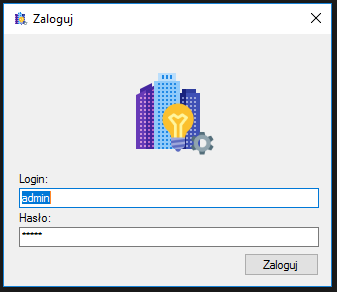
\includegraphics{okno_logowania}
\end{figure}
Po pozytywnym przejściu procesu logowania, użytkownik zostaje przeniesiony do głównego okna aplikacji. Składa się ono z panelu z mapą, panelu wyboru trybu wyświetlania lokalizacji użytkowników oraz przycisku przejścia do konfiguracji.
\begin{figure}[H]			
	\centering
	\caption{Główne okno aplikacji administracyjnej}
	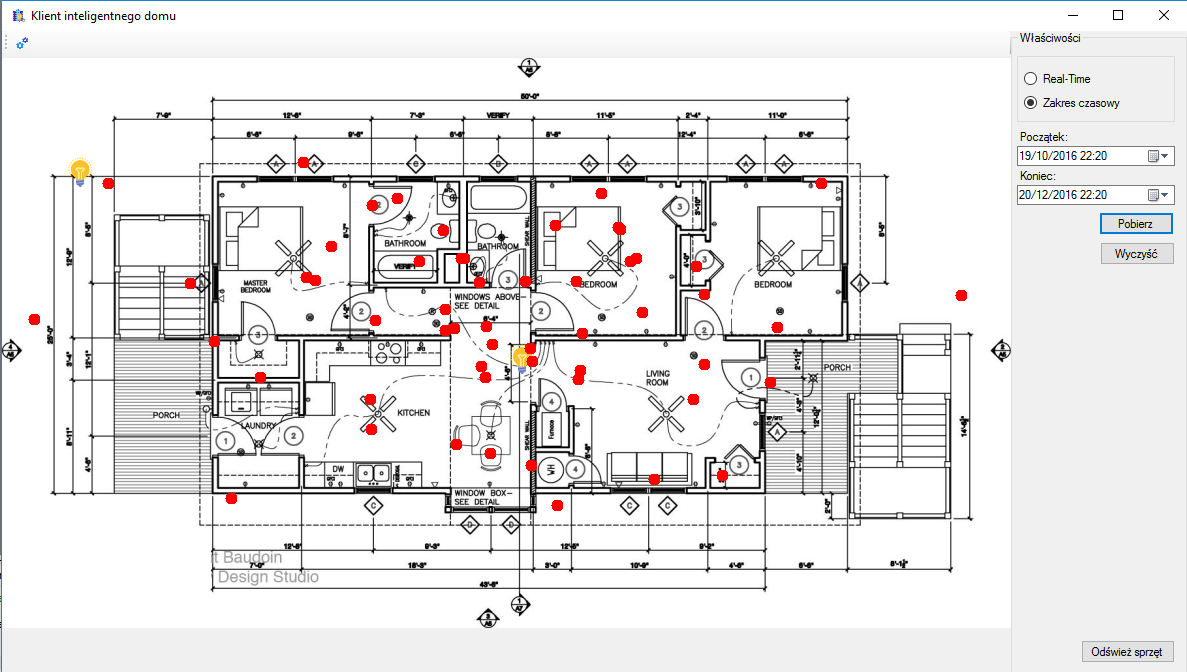
\includegraphics[width=1.0\textwidth]{okno_glowne}
\end{figure}
\subsubsection{Główne okno}
W głównym panelu wyświetlana jest mapa systemu, do której ścieżka określona jest w pliku konfiguracyjnym 'conf.xml'. Jedynym wymaganiem co do mapy jest to, aby była ona plikiem graficznym. Mapa jest skalowalna - każda zmiana wielkości okna powoduje dopasowanie się obrazka do nowego panelu. To samo dotyczy wyświetlanych wewnątrz elementów. Na mapę nanoszone są urządzenia sterowane oraz lokalizacje użytkowników mobilnych. Urządzenia oznaczane są symbolem ich kategorii, zaś użytkownicy reprezentowani są przez czerwone kropki.\\
Lokalizacje urządzeń pobierane są podczas załadowania aplikacji (jednak po poprawnym przejściu procesu logowania) oraz automatycznie wyświetlane. Z racji tego, iż zmiany w konfiguracji urządzeń przez innych użytkowników administracyjnych nie odświeżają ikon na mapie, w prawym dolnym rogu aplikacji znajduje się przycisk, którego naciśnięcie spowoduje ponowne pobranie z serwera lokalizacji sprzętów sterowanych oraz przerysowanie symboli na mapie.\\
Lokalizacje użytkowników mobilnych mogą być wyświetlane w dwóch trybach:
\begin{itemize}
	\item w czasie rzeczywistym - aplikacja administracyjna zgłasza na serwerze chęć zapisania się na subskrypcję lokalizacji. Dzięki temu, za każdym razem, jak serwer ustali lokalizację użytkownika, zostaną o tym powiadomione wszystkie zalogowane aplikacje administracyjne. Punkty oznaczające użytkownika wyświetlane są na okres 4 sekund.
	\item w formie skumulowanej - administrator wysyła na serwer zakres czasowy, dla którego chce wyświetlić pozycje użytkowników. Aplikacja serwerowa pobiera lokalizacje z bazy, a następnie wysyła je spowrotem do klienta, na którym zostają wyświetlone. Punkty oznaczające użytkownika wyświetlane są bez określonego okresu ważności.
\end{itemize}
Przejście pomiędzy trybami powoduje usunięcie zachowanych w pamięci lokalizacji.\\
Punkty reprezentujące użytkowników oraz ikony sprzętów sterowanych są skalowane, aby realistycznie odwzorowywać swoją rzeczywistą pozycję. Wykorzystuje się do tego podane podczas konfiguracji wielkości rzeczywistego systemu.\\
Jeżeli stosunek wysokości mapy do jej szerokości jest większy niż stosunek wysokości panelu wyświetlającego mapę do jego szerokości, pozycję ikony w panelu oblicza się na podstawie wzoru:
\begin{equation}
\left\{
\begin{array}{l}
x = \frac{rzecz\_lok\_urz\_x}{rzecz\_szer\_mapy} * szer\_pan\_mapy \\
y = \frac{(rzecz\_lok\_urz\_y}{rzecz\_wys\_mapy} * wys\_przel\_mapy + wys\_marg 
\end{array}
\right.
\end{equation}
gdzie:
\begin{itemize}
	\item $x$ i $y$ oznaczają współrzędne w panelu mapy
	\item $rzecz\_lok\_urze\_x$ i $rzecz\_lok\_urze\_y$ to fizyczne współrzędne użytkownika mobilnego lub urządzenia sterowanego
	\item $rzecz\_szer\_mapy$ i $rzecz\_wys\_mapy$ to rzeczywiste wymiary prostokąta, wewnątrz którego znajduje się system
	\item $szer\_pan\_mapy$ jest to szerokość panelu wyświetlającego mapę (w tym wypadku szerokość mapy i szerokość panelu jest taka sama)
	\item $wys\_przel\_mapy$ to wysokość mapy. W tym wypadku wysykość mapy nie jest równa wysokości panelu - aby zachować realistyczne proporcję, powyżej i poniżej obrazku mapy dodany jest margines. Wysokość mapy obliczana jest ze wzoru:
	\begin{equation}
	wys\_przel\_mapy = \frac{szer\_pan\_mapy * wys\_obraz\_mapy}{szer\_obraz\_mapy}
	\end{equation}
	w którym $wys\_obraz\_mapy$ i $szer\_obraz\_mapy$ to wymiary obrazka mapy, określone w pikselach.
	\item $wys\_marg$ to wysokość marginesu, jaki musi zostać dodany, aby zachować proporcję mapy. Obliczny jest ze wzoru:
	\begin{equation}
	wys\_marg = \frac{wys\_pan\_mapy - wes\_przel\_mapy}{2}
	\end{equation}
\end{itemize}
W przypadku, jeżeli stosunek wysokości mapy do jej szerokości jest niższy niż stosunek wysokości panelu wyświetlającego mapę do jego szerokości, obliczenia wykonuje się analogicznie, ale z tą różnicą, że w tym wypadku to wysokość mapy będzie równa wysokości panelu i dlatego to faktyczna szerokość mapy w oknie oraz szerokość bocznych marginesów muszą zostać wyliczone.
\subsubsection{Okno konfiguracji}
Wciśnięcie przycisku 'Konfiguracja' (reprezentowane w oknie jako ikona dwóch trybów), otwiera osobne okno, pozwalające na konfigurację kluczowych elementów systemu.\\
Pierwszy panel w oknie konfiguracji pozwala na edycję fizycznej wielkości systemu oraz danych na temat routerów (umożliwia również ich dodawanie oraz usuwanie).
W dolnej części okna wyświetlone są wszystkie zarejestrowane routery. Wciśnięcie wybranego z nich powoduje przejście do trybu edycji - pola edycji routerów zostaną wypełnione danymi wybranego urządzenia.
\begin{figure}[H]			
	\centering
	\caption{Panel edycji danych routerów}
	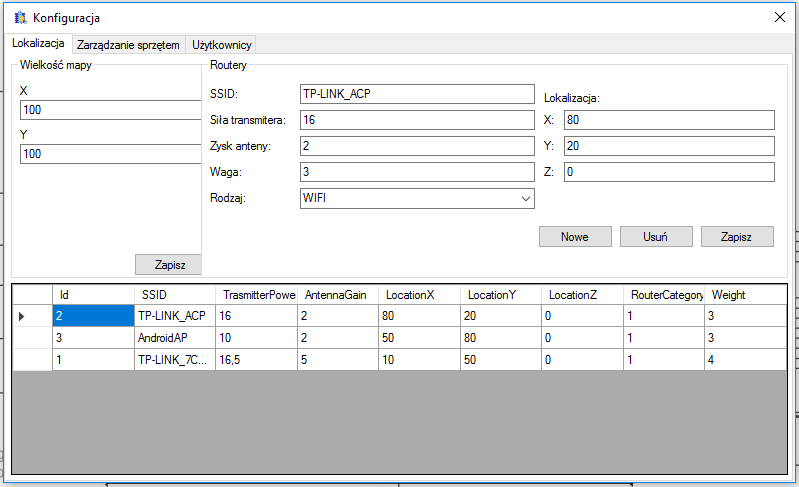
\includegraphics[width=1.0\textwidth]{panel_konf_router}
\end{figure}
Poza polami wymaganymi do lokalizacji użytkownika, którymi są:
\begin{itemize}
	\item lokalizacja routera - współrzędne X, Y, Z oraz SSID
	\item zysk anteny
	\item siła transmitera
\end{itemize}
aplikacja pozwala dodatkowo na zadeklarowanie typu sygnału wysyłanego przez urządzenie. Ma to wpływ na sposób obliczania odległości do użytkowników, ale także na wartość początkową wagi przydzielonej temu transmiterowi. Wagę można zmienić ręcznie, ale trzeba pamiętać, że musi się znaleźć w zakresie <1:4>.\\
Drugi panel pozwala na definiowanie i edycję urządzeń sterowanych.
\begin{figure}[H]			
	\centering
	\caption{Panel edycji urządzeń sterowanych}
	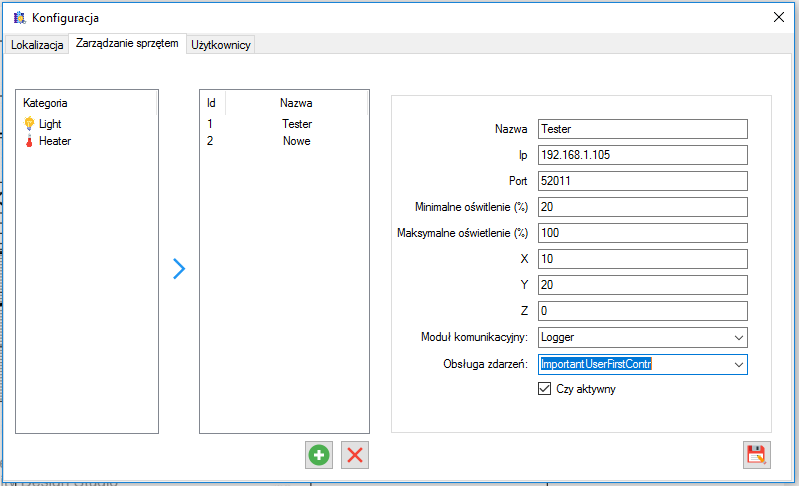
\includegraphics[width=1.0\textwidth]{panel_konf_ster}
\end{figure}
Wszystkie urządzenia zarejestrowane w systemi podzielone są na kategorie. Dostępne kategorie przechowywane są w bazie danych i stamtąd są pobierane, kiedy aplikacja klientowa wyśle żądanie na serwer. Wybranie kategorii z lewego panelu powoduje pobranie z serwera wszystkich urządzeń, które należą do wybranej kategorii. Do każdej kategorii przydzielona jest inna akcja w kontrolerze ConfController na serwerze - przykładowo, dla urządzeń oświetleniowych, jest to akcja GetLightDevices.\\
Aby przejść do widoku wyświetlania i edycji danych urządzenia, należy wybrać interesującą nas pozycję ze środkowego panelu. Powoduje to pojawienie się w prawym panelu formularza z danymi danego urządzenia. Formularze są tworzone dynamicznie, a rodzaj i ilość ich pól zależne są od kategorii urządzenia. Dla urządzenia z kategorii 'Światło', dostępne są następujące pola:
\begin{itemize}
	\item lokalizacji - współrzędne XYZ urządzenia. pozwalające umiejscowić je w rzeczywistym środowisku
	\item adres ip i port - pozwalają na komunikację z urządzeniem
	\item nazwa - pozwala użytkownikom odróżniać urządzenia między sobą
	\item minimalne i maksymalne oświetlenie - zakres, określony w procentach, z którego może korzystać system podczas sterowania urządzeniem. W przypadku sterowania w interwałach czasowych, minimalne oświetlenie przydzielane jest w sytuacji, gdy, w podanym okresie czasu, obok urządzenia nie przeszedł żaden użytkownik. Analogicznie, maksymalne oświetlenie przydzielane jest, gdy wszystkie obliczone lokalizacje użytkowników znajdowały się w niedalekiej odległości od sterowanego urządzenia
	\item moduł komunikacyjny - określa sterownik, sposób komunikacji serwera z urządzeniem. Moduły komunikacyjne definiowane są w bazie danych, a związane z nimi klasy obsługujące muszą zostać dodane do kodu serwera
	\item obsługa zdarzeń - nazwa modułu, który na bieżąco steruje urządzeniem, w zależności od lokalizacji użytkowników zlokalizowanych w bliskiej odległości. Z modułem związana jest klasa, która obsługuje przypisany do urządzenia moduł
\end{itemize}
Panel udostępnia przyciski, które pozwalają na zapis wprowadzonych zmian, jak również dodanie lub usunięcie urządzenia.\\
Ostatni panel to panel użytkowników. Są to osoby, które korzystały z aplikacji mobilnej, a ich pozycja została chociaż raz obliczona.
\begin{figure}[H]			
	\centering
	\caption{Panel edycji urządzeń sterowanych}
	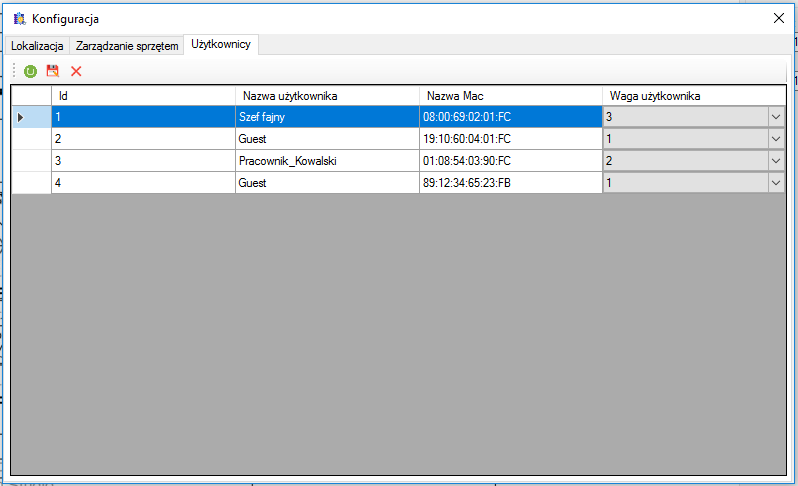
\includegraphics[width=1.0\textwidth]{panel_konf_users}
\end{figure}
Okno składa się z tabeli, w której znajdują się zapisani użytkownicy oraz przycisków:
\begin{itemize}
	\item odświeżania danych
	\item zapisania wszystkich użytkowników
	\item usunięcia wybranego w tabeli użytkownika
\end{itemize}
Widok pozwala na podglądnięcie użytkowników oraz na zmianę ich nazwy oraz wagi. Nazwa pozwala na rózróżnianie użytkowników w sposób łatwiejszy niż po adresie MAC. Waga odgrywa kluczową rolę podczas obliczania parametrów do sterowania urządzeniami - czym wyższa waga użytkownika, tym większe ma on znaczenie dla urządzenia, w którego pobliżu znajduje się obliczona lokalizacja. Dodatkowo, pojawienie się użytkownika o określonej wadze może mieć wpływ na zajście zdarzenia, zdefiniowanego dla urządzenia. Wagi przyjmują wartość od 0 (użytkownik o najniższym priorytecie, nie brany pod uwagę podczas określania parametrów) do 4 (użytkownik o najwyższym priorytecie).
\subsection{Wyświetlanie lokalizacji użytkowników} W trybie wyświetlania lokalizacji w czasie rzeczywistym, aplikacja musi wyświetlać uzyskane dane bez odświeżania panelu czy ingerencji użytkownika. W związku z tym potrzebne było wprowadzenie mechanizmu opartego na osobnym wątku. Klasą zarządzającą rysowanie punktów jest PointPainter. W wątku wykonuje się metoda tej klasy, DrawPoint(), zawierająca nieskończoną pętlę, usypianą na 0,5 sekundy przy każdym przejściu. Wątek ma dostęp do listy punktów, które powinien wyświetlić. Lista uzupełniania jest przez obiekt klasy HttpServerThread, na podstawie notyfikacji przychodzących z serwera. Każdy wpis na liście ma informacje o lokalizacji (współrzędne XY) oraz dacie ważności danego punktu. Punkty stworzone na podstawie notyfikacji z serwera mają okres ważności równy 4 sec, za to punkty wyświetlane w sposób skumulowany mają datę ważności ustawioną na wartość null (co oznacza, że są wyświetlane dopóki nie zostanie wywołana komenda wyczyszczenia mapy).
\begin{figure}[H]			
	\centering
	\caption{Schemat rysowania elementów systemu na mapie}
	\includegraphics[width=1.0\textwidth]{obrazek_pointPainter}
\end{figure}
Metoda wyświetlająca punkty nie rysuje ich bezpośrednio na wyświetlonej mapie, ponieważ odświeżanie wymagałoby ponownego przerysowania nie tylko punktów, ale i całej mapy. Mogłoby to powodować opóźnienia w płynności wyświetlania, a wiązałoby się z tym nieprzyjemne dla oka 'mruganie' mapy. Dlatego, punkty nanoszone są na przeźroczysty obrazek, który później wyświetlany jest na warstwie wyświetlającej punkty. Zanim jednak na obrazku zostaną naniesione lokalizację użytkowników, klasa PointPainter zaznacza na przeźroczystej warstwie urządzenia sterowane, rysując odpowiednią ikonę kategorii danego sprzętu. Dodatkowo, ponieważ metoda rysująca punkty działa na innym wątku niż panel zawierający mapę, wyświetlenie punktów nie może być wywołane bezpośrednio z poziomu klasy PointPainter. Z tego powodu, funkcja rysująca obraz z punktami i ikonami urządzeń na mapie zostaje opakowana w delegatę (typ danych przechowujący funkcję), a następnie referencja do niej zostaje wstawiona jako parametr funkcji Control.Invoke(delegate), dzięki czemu panel sam wywoła przekazaną mu jako parametr funkcję podczas kolejnego wykonywania się jego wątku.
\chapter{Testy systemu}
\section{Lokalizowanie użytkownika}
\section{Monitorowanie i konfiguracja systemu}
W celu przetestowania w działania aplikacji klienckiej, została utworzona osobna aplikacja, której celem było symulowanie aplikacji mobilnej. Aplikacja testująca składała się z panelu, którego rozmiar był dostosowany do wielkości obszaru pracy systemu. W momencie, jak użytkownik kliknął wewnątrz panelu, pozycja myszki została przeliczana na rzeczywistą pozycję w systemie. Następnie aplikacja, przy użyciu danych na temat statycznych transmiterów, obliczała dystans, a następnie siłę sygnału do każdego z zarejestrowanych routerów i Beaconów. Tak obliczone dane wysyłane były na serwer protokołem HTTP, na adres odpowiedniego kontrolera. Tak sformatowane zgłoszenie było rozpatrywane przez serwer tak samo, jakby informacje były wysłane przez aplikację mobilną.\\
\section{Podsumowanie}
Celem pracy było stworzenie systemu, który określa położenie użytkownika w trzech wymiarach na podstawie siły sygnału znanych ruterów, stałych urządzeń Bluetooth (np Beacony) oraz dynamicznie zmieniających się sił sygnałów Bluetooth innych użytkowników systemu. Obliczone lokalizacje miały być przechowywane oraz przedstawienie ich na mapie budynku w sposób łatwy do analizy. Dodatkowo, celem było opracowanie algorytmu, który na podstawie określonych warunków oraz mapy przepływu zarządza wybranymi urządzeniami podłączonymi do systemu.



% itd.
% \appendix
% \include{dodatekA}
% \include{dodatekB}
% itd.

\printbibliography

\end{document}
